\documentclass[journal]{IEEEtran}
\usepackage[a5paper, margin=10mm]{geometry}
%\usepackage{lmodern} % Ensure lmodern is loaded for pdflatex
\usepackage{tfrupee} % Include tfrupee package


\setlength{\headheight}{1cm} % Set the height of the header box
\setlength{\headsep}{0mm}     % Set the distance between the header box and the top of the text


%\usepackage[a5paper, top=10mm, bottom=10mm, left=10mm, right=10mm]{geometry}

%
\setlength{\intextsep}{10pt} % Space between text and floats

\makeindex


\usepackage{cite}
\usepackage{amsmath,amssymb,amsfonts,amsthm}
\usepackage{algorithmic}
\usepackage{graphicx}
\usepackage{textcomp}
\usepackage{xcolor}
\usepackage{txfonts}
\usepackage{listings}
\usepackage{enumitem}
\usepackage{mathtools}
\usepackage{gensymb}
\usepackage{comment}
\usepackage[breaklinks=true]{hyperref}
\usepackage{tkz-euclide} 
\usepackage{listings}
\usepackage{multicol}
\usepackage{xparse}
\usepackage{gvv}
%\def\inputGnumericTable{}                                 
\usepackage[latin1]{inputenc}                                
\usepackage{color}                                            
\usepackage{array}                                            
\usepackage{longtable}                                       
\usepackage{calc}                                             
\usepackage{multirow}                                         
\usepackage{hhline}                                           
\usepackage{ifthen}                                               
\usepackage{lscape}
\usepackage{tabularx}
\usepackage{array}
\usepackage{float}
\usepackage{ar}
\usepackage[version=4]{mhchem}


\newtheorem{theorem}{Theorem}[section]
\newtheorem{problem}{Problem}
\newtheorem{proposition}{Proposition}[section]
\newtheorem{lemma}{Lemma}[section]
\newtheorem{corollary}[theorem]{Corollary}
\newtheorem{example}{Example}[section]
\newtheorem{definition}[problem]{Definition}
\newcommand{\BEQA}{\begin{eqnarray}}
\newcommand{\EEQA}{\end{eqnarray}}

\theoremstyle{remark}


\begin{document}
\bibliographystyle{IEEEtran}
\onecolumn

\title{1.5.15}
\author{INDHIRESH S- EE25BTECH11027}
\maketitle


\renewcommand{\thefigure}{\theenumi}
\renewcommand{\thetable}{\theenumi}

\textbf{Question} The midpoint of the line segment joining $A(2a, 4)$ and $B(-2, 3b)$ is $(1, 2a + 1)$. Findthe values of a and b.\\
\textbf{Solution}:\\
Let us solve the given equation theoretically and then verify the solution computationally. \\
From the given data,
\begin{align}
\vec{A}= \myvec{2a\\4} , \vec{B}=\myvec{-2\\3b}
\end{align}
Let the midpoint of points A and B be C. where,
\begin{align}
    \vec{C}=\myvec{1\\2a+1}
\end{align}
We know that the midpoint formula for the points A and B is
\begin{align}
    \vec{C}=\frac{\vec{A}+\vec{B}}{2}
    \end{align}
\begin{align}
    \myvec{1\\2a+1}=\frac{\myvec{2a\\4}+\myvec{-2\\3b}}{2}
\end{align}
\begin{align}
    \myvec{1\\2a+1}=\frac{\myvec{2a-2\\4+3b}}{2}
\end{align}
\begin{align}
    \myvec{1\\2a+1}=\myvec{a-1\\2+\frac{3b}{2}}
\end{align}
From Eq.6 we can say that:
\begin{align}
    2a+1=2+\frac{3b}{2}
\end{align}
\begin{align}
    2a=1+\frac{3b}{2}
\end{align}
\begin{align}
    4a=2+3b
\end{align}
\begin{align}
    4a-3b=2
\end{align}
Let P=\myvec{C-A& B-A }. A,B and C lies in the same line so they are collinear. So,
\begin{align}
   rank\myvec{C-A&B-A}=1\\
   rank\myvec{1-2a&-2-2a\\
   2a-3&3b-4}=1
\end{align}
Now by applying the row operation for the matrix P\\
$R_2\longrightarrow R_2-(\frac{2a-3}{1-2a})R_1$

\begin{align}
    P=\myvec{1-2a&-2-2a\\0&3b-4-(\frac{2a-3}{1-2a})(-2-2a)}
\end{align}
For the rank to be 1 , all entries of $R_2$ should be zero. so,
\begin{align}
3b-4-(\frac{2a-3}{1-2a})(-2-2a)=0
\end{align}
\begin{align}
    \frac{(3b-4)(1-2a)+(2a-3)(2+2a)}{1-2a}=0
\end{align}
\begin{align}
    \frac{4a^2-6ab+6a+3b-10}{1-2a}=0
\end{align}
\begin{align}
    4a^2-6ab+6a+3b-10=0
\end{align}
From Eq.10 we can get
\begin{align}
    b=\frac{4a-2}{3}
\end{align}
Now substituting 'b' in Eq.17, we get:
\begin{align}
2a^2-7a+6=0
\end{align}
By solving the above quadratic equation we get:
\begin{align}
a=2,\frac{3}{2}
\end{align}
By substituting the value of 'a' in Eq.18 we get:
\begin{align}
b=2,\frac{4}{3}
\end{align}
But when $a=\frac{3}{2}$ and $b=\frac{4}{3}$ it does not satisfies the Eq.3\\
So the final value of a and b are:
\begin{align}
    a=2\;and\;b=2
\end{align}


From the figure it is clearly verified that the theoretical solution matches with the computational solution.\\
\begin{figure}[h]
    \centering
    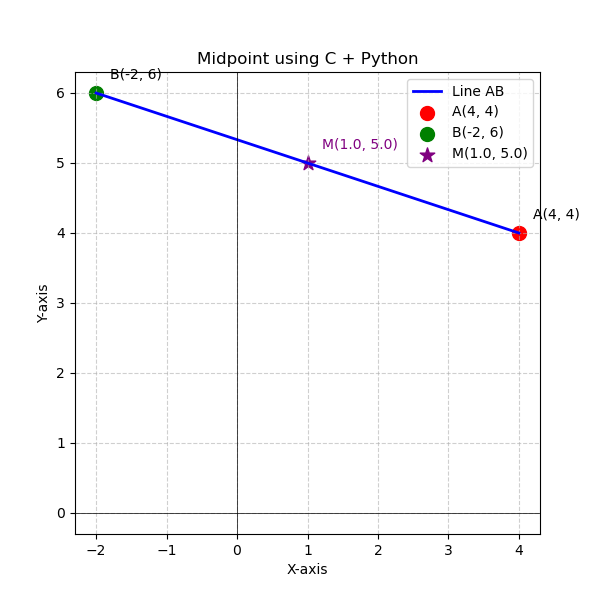
\includegraphics[height=0.5\textheight, keepaspectratio]{figs/figure1.png}
    \label{figure_1}
\end{figure}

\end{document}